
\documentclass[twoside]{article}
\setlength{\oddsidemargin}{0.25 in}
\setlength{\evensidemargin}{0.25 in}
\setlength{\topmargin}{-0.6 in}
\setlength{\textwidth}{6.5 in}
\setlength{\textheight}{8.5 in}
\setlength{\headsep}{0.75 in}
\setlength{\parindent}{0 in}
\setlength{\parskip}{0.1 in}


%
% ADD PACKAGES here:
%

\usepackage{amsmath,amsfonts,graphicx,amsthm,amssymb}
\usepackage{hyperref}
\usepackage[ruled,vlined]{algorithm2e}
\usepackage{cancel}
\usepackage{multicol}
\usepackage{float}


\hypersetup{
    colorlinks=true,
    linkcolor=blue,
    filecolor=magenta,
    urlcolor=blue,
}

%
% The following macro is used to generate the header.
%
\newcommand{\customheader}[3]{
   \pagestyle{myheadings}
   \thispagestyle{plain}
   \newpage
   \setcounter{page}{1}
   \noindent
   \begin{center}
   \framebox{
      \vbox{\vspace{2mm}
    \hbox to 6.28in { {\bf EE 381V: Special Topics on Unsupervised Learning
        \hfill Spring 2018} }
       \vspace{6mm}
       \hbox to 6.28in { {\Large \hfill #1  \hfill} }
       \vspace{6mm}
       \hbox to 6.28in { {\it Professor: #2 \hfill Students: #3} }
      \vspace{2mm}}
   }
   \end{center}
   \vspace*{4mm}
}

%
% Convention for citations is authors' initials followed by the year.
% For example, to cite a paper by Leighton and Maggs you would type
% \cite{LM89}, and to cite a paper by Strassen you would type \cite{S69}.
% (To avoid bibliography problems, for now we redefine the \cite command.)
% Also commands that create a suitable format for the reference list.
%\renewcommand{\cite}[1]{[#1]}
%\def\beginrefs{\begin{list}%
        %{[\arabic{equation}]}{\usecounter{equation}
         %\setlength{\leftmargin}{2.0truecm}\setlength{\labelsep}{0.4truecm}%
%         \setlength{\labelwidth}{1.6truecm}}}
%\def\endrefs{\end{list}}
%\def\bibentry#1{\item[\hbox{[#1]}]}

%Use this command for a figure; it puts a figure in wherever you want it.
%usage: \fig{NUMBER}{SPACE-IN-INCHES}{CAPTION}
\newcommand{\indep}{\rotatebox[origin=c]{90}{$\models$}}
\newcommand{\fig}[3]{
			\vspace{#2}
			\begin{center}
			Figure \thelecnum.#1:~#3
			\end{center}
	}
% Use these for theorems, lemmas, proofs, etc.
\theoremstyle{definition}
\newtheorem{theorem}{Theorem}
\newtheorem{example}[theorem]{Example}
\newtheorem{lemma}[theorem]{Lemma}
\newtheorem{proposition}[theorem]{Proposition}
\newtheorem{claim}[theorem]{Claim}
\newtheorem{corollary}[theorem]{Corollary}
\newtheorem{note}[theorem]{Note}
\newtheorem{definition}[theorem]{Definition}

% **** IF YOU WANT TO DEFINE ADDITIONAL MACROS FOR YOURSELF, PUT THEM HERE:

\newcommand{\norm}[2]{\left\lVert #1 \right\rVert_{#2}}

%*****--------------------------------------------------------------------

\begin{document}
%\lecture{**Document-Title**}{**DATE**}{**Professor**}{**Students**}
\customheader{Attacking Robust Manifold Defense}{Alex Dimakis}{Kwon Jeongyeol, Dany Haddad, Justin Lewis}

\section{Synopsis}
The success of adversarial attacks has brought increased scrutiny regarding the robustness of neural networks. A variety of defense methods have been proposed, some of the more successful techniques are closely  related to the Invert and Classify (INC) approach. INC uses a well-trained generative model to project a potentially adversarial image
onto the manifold of natural images. This sister-image can now be safely classified as it no longer
contains adversarial components which are far from the manifold. This process is not directly differentiable and as a result is seemingly
difficult to attack. In response, our proposal is the following. Given the well-trained GAN used for
the Manifold Defense, train a matching encoder. Together, the GAN and encoder form an autoencoder which
is now directly differentiable and susceptible to adversarial attack. 

\section{Background}
The following subsections will introduce basic notation for deep learning frameworks.
Additionally the notion of adversarial attack and training will be made clear. 

\subsection{Notation}

Let our dataset be denoted by $\{\mathcal{X},\mathcal{Y}\}$, a set of images $\mathcal{X}$ and corresponding
class labels $\mathcal{Y}$


Classifier: $\mathcal{C}_{\theta}$ 

GAN: generator $\mathcal{G}_{\phi}$ and discriminator $\mathcal{D}_{\psi}$

AE: encoder $\mathcal{E}_{\alpha}$ and decoder $D_\beta$

$x$: a natural image

$x_{adv}$: an adversarial image

\iffalse

\begin{multicols}{3}
%Column 1
Classifier: $\mathcal{C}_{\theta}$ 
\columnbreak
%Column 2
GAN: generator $\mathcal{G}_{\phi}$ and discriminator $\mathcal{D}_{\psi}$
\columnbreak
%Column 3
AE: encoder $\mathcal{E}_{\alpha}$ and decoder $D_\beta$
\end{multicols}


Given dataset $\{\mathcal{X},\mathcal{Y}\}$, a set of images $\mathcal{X}$ and corresponding
class labels $\mathcal{Y}$, a classifier $\mathcal{C}_{\theta}$ is tasked with correctly labeling the 
images in a held-out training set.

A Generative Adversarial Network with generator $\mathcal{G}_{\phi}$ and discriminator $\mathcal{D}_{\psi}$, 
is tasked with learning the underlying structure of $\mathcal{X}$ in an unsupervised fashion. 
\fi

\subsection{Adversarial Attacks and Training}
The notion of adversarial attacks is a phenomenon brought to light in the context of deep learning by Goodfellow et al. \cite{2014arXiv1412.6572G}. In essence,
they argue that deep learning classifiers are less robust than their celebrated performance assumes and are susceptible to attack from an adversarial user.
Given image $x$ with correct label $y$ and trained classifier $\mathcal{C_{\theta}}$ with loss function
$L(x,y;\theta)$, a canonical adversarial attack is conducted as follows:

\begin{equation*}
\begin{aligned}
& \underset{\delta}{\text{maximize}}
& & L(x+\delta,y;\theta) \\
& \text{subject to}
& & \norm{\delta}{p} \leq \epsilon
\end{aligned}
\end{equation*}

Plainly said, find adversarial image $x_{adv} = x + \delta$ within an $\epsilon$ sized $\ell_p$ ball around the
original image which fools the classifier the most. Commonly, this optimization problem is approximately solved using
one of two approaches: Fast Gradient Sign Method (FGSM) and projected gradient descent (PGD). It has been empirically
verified that FGSM attacks are less effective at fooling a classifier than PGD approaches \cite{madry}. Note, a suitable
loss function $L(x,y;\theta)$ might be cross-entropy loss for multi-label classification. 

%There are a number of different environment assumptions that can be made to result in different attack models.
%The above attack is a white-box, non-targeted attack.

In order to defend against adversarial attacks, a number of defense strategies have been employed \cite{2018arXiv180200420A}.
The most straightforward defense strategies introduce adversarial examples $\mathcal{X}_{adv}$ into the set of training images
$\mathcal{X}$, which allows the network to learn to correctly classify even these examples. Other methods try to 
"detect" adversarial examples. Essentially, these defense strategies give no clear guarantees and the process of
attack-defend becomes an arms-race. 

\section{Invert and Classify Defense}
The defense strategy of particular interest to our proposal is the Invert and Classify (INC) approach as introduced by \cite{2017arXiv171209196I} and a very similar technique developed by \cite{pixel}. As mentioned before, INC leverages the strong representation power
of GANs. The idea is to project an adversarial image onto the range of a GAN and classify this 'cleaned' image.
This is done using gradient descent. If the GAN has approximated the manifold of natural images well enough, and
the gradient method projects onto the manifold well enough, then the INC strategy is feasible.

\begin{center}
    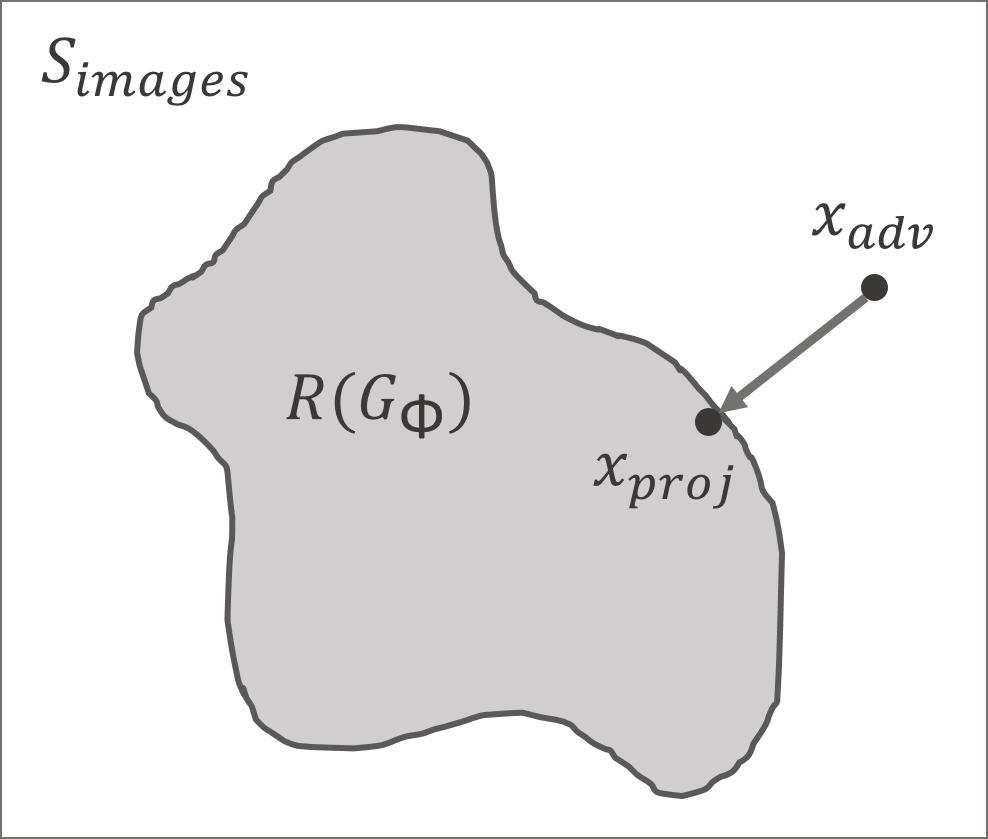
\includegraphics[scale=0.3]{./projection_diagram.png}
\end{center}

$S_{images}:$ the space of all images

$R(G_{\phi}):$ the range of the GAN

\section{Attacking INC}
Similar to the Backward Pass Differentiable Approximation (BPDA) method of Athalye et al., we propose to attack the INC defense mechanism by building a differentiable approximation for the process of projecting onto the manifold of natural images. Using this approximation, we can evaluate a gradient and perform gradient based attacks (FGSM and PGD). We learn this approximation by training an encoder that corresponds to the generative model used in the INC process. In this way, passing an image through the encoder and then the generative model will give us an image on the learned manifold which will serve as an approximation to the projection process. To learn this encoder, we minimize the following loss with respect to the parameters of the encoder, $E$:
\begin{equation}
    \mathbb{E} [||E(G(Z)) - Z||_2^2]
\end{equation}


\subsection{Preliminary Results}
We ran some experiments using the MNIST dataset. The adversarial images $\mathcal{X_a}$ were generated
through FGSM attacks on the unprotected classifier $\mathcal{C}_{\theta}$. The classification accuracy results
are presented below.

\begin{itemize}
    \item Clean test data: 98\%
    \item Adversarial test set using FGSM and $\epsilon = 0.2$: 19\%
    \item Adversarial test set against INC protected classifier: 87\%
    \item Adversarial test set against fitted encoder protected classified: 75\%
\end{itemize}

Using our BPDA style attack on an INC protected classifier (differentiating through an encoder fitted to the GAN used in the INC process) we did not arrive at the results that we had hoped for: the accuracy of the INC protected classifier remained at 93\%. Shown below are the original images, the adversarial examples created via FGSM and the images resulting from the autoencoding process.

\begin{figure}[H]
\centering
\begin{tabular}{ccc}
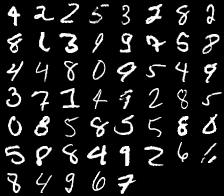
\includegraphics[width=2in]{cl_original.png} &
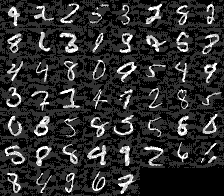
\includegraphics[width=2in]{cl_adversarial.png} &
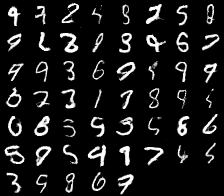
\includegraphics[width=2in]{cl_reconstr.png}
\end{tabular}
\caption{Some failure cases in MNIST test data, the adversarial examples created via FGSM and the images resulting from the autoencoding process}
\end{figure}

% insert table showing classification error under different circumstances for mnist

% eps - 0.2 (FGSM on classifier solely)
% clean clasisifcation - 98%
% adversarial classification (using FGSM or PGD) - 19%
% GAN defended classification - 87%
% Fitted encoder defense classification - 75%

% attack using fitted encoder on gan protected classifier - later added
% (but typically 93%, while it drop encoder-only defense's performance down to 56%)

% insert image of fitted encoder method and projection onto gan (for mnist)


\subsection{Paths Forward}
It is likely that the reason this attack fails is that the encoder does not serve as a close enough approximation of the projection step. It would be interesting to see if for certain synthetic datasets our attack will be effective.

Additionally, we have also considered using the fitted encoder to bootstrap an attack which unrolls the projection process.

\section{Using Fitted Encoder to Improve INC}
Does the failure of the attack using the fitted encoder mean that the fitted encoder is useless? During experiment, we observed interesting phenomenon. 

\subsection{Learned Encoder vs. Projection}
As stated earlier, projection step in INC solves the optimization problem that minimizes $||G(z) - X||_2$. However, the non-convex nature of this problem requires us to start over many randomly initialized points and pick the best one. It might be computationally very expensive to iterate over and over again until getting a satisfactory reconstruction, sometimes making this defense mechanism impractical to use, as suggested in their experiment with CIFAR-10 data. 

From our experiment, we observed that a latent point mapped by fitted encoder becomes a very good starting point to launch the optimization procedure. We speculate that the learned encoder at least gives us very good reference for each test image and even for corrupted image.

\begin{figure}[H]
\centering
\begin{tabular}{ccc}
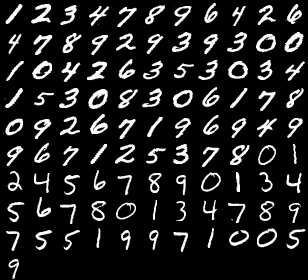
\includegraphics[width=2in]{original_d.png} &
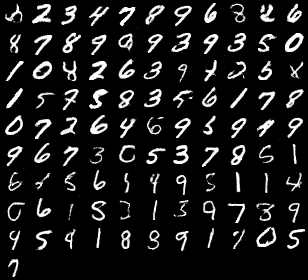
\includegraphics[width=2in]{reconstr_random_z.png} &
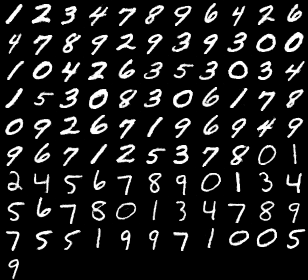
\includegraphics[width=2in]{reconstr_encoded.png}
\end{tabular}
\caption{Some MNIST test images, reconstruction from random z, and encoded z.}
\end{figure}


%*****--------------------------------------------------------------------
\bibliographystyle{plain}
\bibliography{ref}

\end{document}